\documentclass{article}
\newtheorem{thm}{Theorem}
\setlength{\oddsidemargin}{0.25in}
\setlength{\textwidth}{6in}
\setlength{\topmargin}{-0.25in}
\setlength{\headheight}{0.3in}
\setlength{\headsep}{0.2in}
\setlength{\textheight}{9in}
\setlength{\footskip}{0.1in}
\usepackage{multirow}
\usepackage{fullpage}
\usepackage{graphicx}
\usepackage{amsthm}
\usepackage{amssymb}
\usepackage{url}
\usepackage{amsfonts}
\usepackage{algpseudocode}
\usepackage{mathtools}

\usepackage{listings}
\usepackage{color}
 
\definecolor{codegreen}{rgb}{0,0.6,0}
\definecolor{codegray}{rgb}{0.5,0.5,0.5}
\definecolor{codepurple}{rgb}{0.58,0,0.82}
\definecolor{backcolour}{rgb}{0.95,0.95,0.92}
 
\lstdefinestyle{mystyle}{
    backgroundcolor=\color{backcolour},   
    commentstyle=\color{codegreen},
    keywordstyle=\color{magenta},
    numberstyle=\tiny\color{codegray},
    stringstyle=\color{codepurple},
    basicstyle=\footnotesize,
    breakatwhitespace=false,         
    breaklines=true,                 
    captionpos=b,                    
    keepspaces=true,                 
    numbers=left,                    
    numbersep=5pt,                  
    showspaces=false,                
    showstringspaces=false,
    showtabs=false,                  
    tabsize=2
}
 
\lstset{style=mystyle}

\begin{document}\title{Project 7: Harp K-Means\\ Cloud Computing\\ Spring 2017}         % Enter your title between curly braces
\author{Professor Judy Qiu }        % Enter your name between curly braces
\date{}
%\date{\today}          % Enter your date or \today between curly braces
\maketitle
\makeatother     % `@' is restored as a "non-letter" character
\pagestyle{plain}
\section*{Goal}
The goal of this project is to familiarize yourself with the concept of map-collective applications. Harp is similar to MapReduce in programming with the exception that it provides collective communication support across map tasks.

\section*{Deliverables}
Zip your source code and output as username\_harp-kmeans.zip. Please submit this file to the Canvas Assignments page.

\section*{Evaluation}
The point total for this project is 20, where the distribution is as follows:
\begin{itemize}
\item Completeness of your code (16 points)
\item Correct output (4 points)
\end{itemize}

\section*{Prerequisites}
\begin{itemize}
\item Before working on Harp K-Means, make sure you can successfully run Harp WordCount following the instructions of Lab 10 (the presentation is in Canvas).
\item Download \textbf{simplekmeans} folder from Canvas assignments under \textbf{B649\_Project7} folder.
\item Copy that folder to \textbf{harp2-project-master/harp2-app/src/edu/iu}
\item Open \textbf{harp2-project-master/harp2-app/build.xml} and add the following line next to where you find other \textbf{include} tags. Note: this is within the \textbf{javac} tag of the \textbf{build.xml}\\
\textbf{\textless include name=``edu/iu/simplekmeans/**'' /\textgreater}
\end{itemize}

\section*{K-Means Clustering Algorithm}
K-Means is a clustering algorithm to partition $n$ observations $(x_1,x_2,..., x_n)$ into $k$ $(\leq n)$ sets $S=\{S_1,S_2,...,S_k\}$ clusters in which each observation belongs to the cluster with the nearest mean of Euclidean distance. The objection function is to minimize the sum of distance functions for each point to centroids, where $\mu_i$ is the mean of points in $S_i$.
\begin{eqnarray*}
\arg\min\limits_S\sum\limits_{i=1}^k\sum\limits_{x\in S_i}{||x-\mu_i||}^2
\end{eqnarray*}
The input is data points (data) and the model is cluster centers (centroids). The problem is computationally difficult (NP-hard); however, there are efficient algorithms via an iterative refinement approach.

\begin{figure}[!htbp]
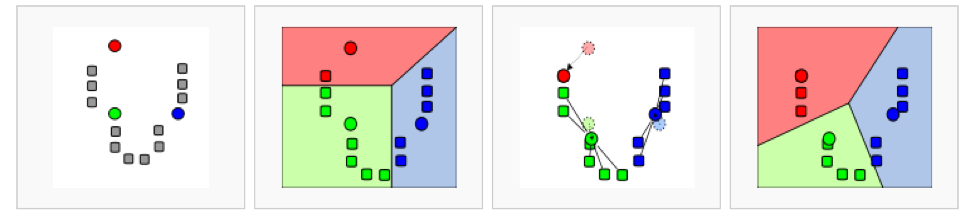
\includegraphics[width=8cm,height=2cm]{p7-1}
\centering
\caption{Image source: https://en.wikipedia.org/wiki/K-means\_clustering}
\end{figure}

\begin{figure}[!htbp]
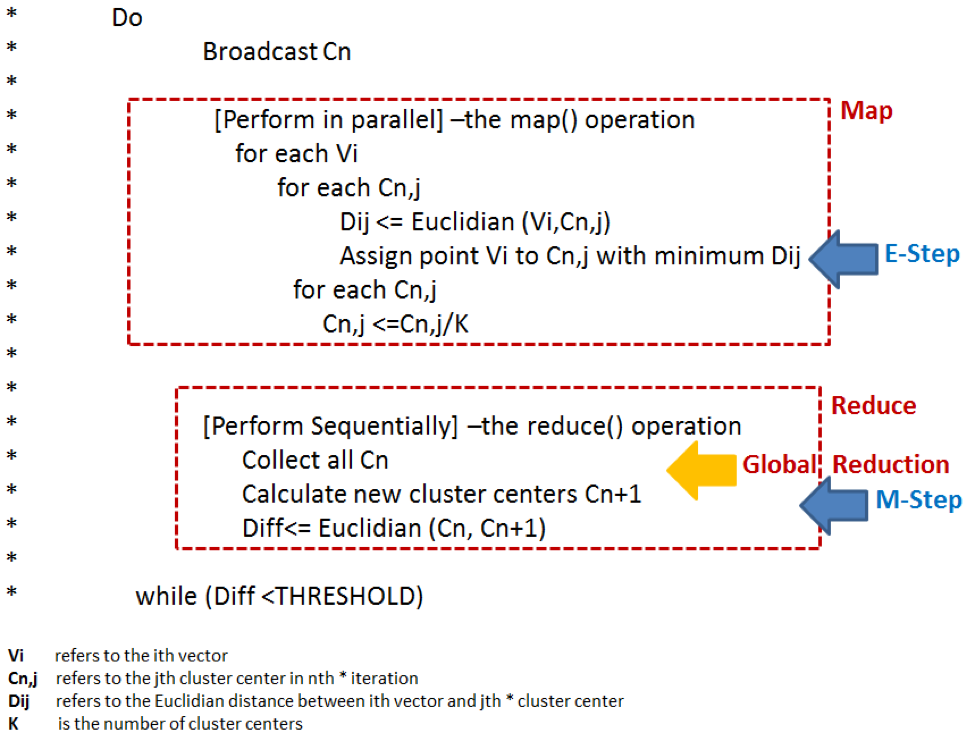
\includegraphics[width=8cm,height=6cm]{p7-2}
\centering
\caption{K-Means Clustering for MapReduce}
\end{figure}

\section*{Harp Data Structure}
The main data structure used for this assignment is ArrTable\textless DoubleArray\textgreater. You can think of  this as a collection of double array objects. Each double array represents a center. For example, if  the centers for your program are 3D, then each array will have $3+1$ (4) elements. The first 3 will be the $x, y, z$ coordinates. The last element is used to store the number of points assigned to this center. 

To retrieve all the centers you can invoke the \textbf{getPartitions()} method on ArrTable  object, which will return a collection of  ArrPartition objects. To retrieve the underlying double array from these ArrPartition objects, you can invoke the \textbf{getArray()} method on ArrPartition object. To figure out the index (ID) of this center you can invoke \textbf{getPartitionID()} method on the same ArrPartition object.

\begin{figure}[!htbp]
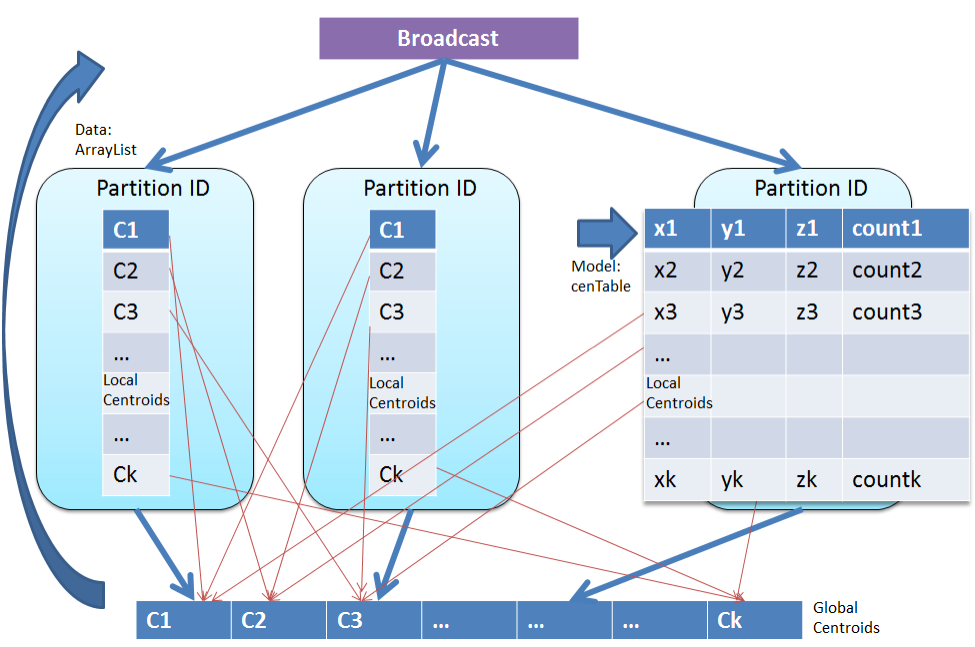
\includegraphics[width=8cm,height=5cm]{p7-3}
\centering
\caption{Parallelization of K-means Clustering}
\end{figure}

\section*{Harp Implementation}
Most of the code is completed for you; your task will be to perform the nearest center finding computation and updating new centers. The code to implement this is in the \textbf{simplekmeans/KmeansMapper.java}

The two functions are listed below.

\textbf{Finding Nearest Center}
\lstinputlisting[language=Java]{FindingNearestCenter.java}

\textbf{Updating Centers}
\lstinputlisting[language=Java]{UpdatingCenters.java}

\section*{Compilation and Running}
\begin{itemize}
\item To compile the code, simply go into \textbf{harp2-project-master/harp2-app} and type \textbf{ant}
\item Then copy the \textbf{harp2-project-master/harp2-app/build/harp2-app-hadoop-2.6.0.jar} to \\
\textbf{\$HADOOP\_HOME}
\item To run the file, use the following command within \textbf{\$HADOOP\_HOME}. This will produce 100 data points and cluster them into 12 clusters. We use 3D points. The program will run 2 parallel map tasks for 20 iterations. Note: you may want to give unique directory names for the last two parameters each time that you test. Otherwise, you may run into issues because of existing directories. Alternatively, you can delete old directories and reuse the same names. 

The folder \textbf{harpkmeans} will be in HDFS. The \textbf{/tmp/simplekmeansdata} will be in your local disk.
\begin{lstlisting}[language=bash]
$ hadoop jar harp2-app-hadoop-2.6.0.jar edu.iu.simplekmeans.KmeansMapCollective 100 12 3 2 20 harpkmeans /tmp/simplekmeansdata
\end{lstlisting}
\item To get the output do the following and look at the part- files as usual.
\begin{lstlisting}[language=bash]
$ hdfs dfs -get harpkmeans/out .
\end{lstlisting}
\end{itemize}

\bibliographystyle{unsrt} 
\end{document}
